Para realizar la medicion de la ganancia del amplificador se debe conectar una carga igual a la que habitualmente se utilizaria en funcionamiento normal, para ello se procedio a dejar el resistor conectado y ajustado tal cual como estaba en el experimento anterior. El valor de ganancia normalmente se expresa en decibeles, por lo tanto es conveniente utilizar instrumentos con escalas en \textbf{dB}, como es el caso del multimetro Univo que también se utilizo en la experiencia anterior.

El multímetro utilizado para esta medición, como ya sea visto en el experimento anterior, puede expresar valores de tensión referenciados a $0.775V$ o \textbf{dBu}. El procedimiento para determinar la ganancia en tensión es, entonces comparar las tensiones de salida y de entrada, y restando ambos valores deberíamos ser capaces de obtener el valor de la ganancia de tensión. Recordando la ecuación de \textbf{dBu} (ecuación \ref{eq::VolReferidoa775mV}).

\begin{equation}\label{eq:Exp4RefGv}
\begin{aligned}
    G_V = GS_{dBu}-GE_{dBu}=&20\cdot\log{\frac{V_s}{0.775V}}-20\cdot\log{\frac{V_e}{0.775V}}\\
                    \\
                    G_V =&20\cdot\log{\frac{V_s/0.775V}{V_e/0.775V}}\\
                    \\
                    G_V =&20\cdot\log{\frac{V_s}{V_e}}
\end{aligned}
\end{equation}
%\begin{equation}
%    GV_{dB}=20\cdot\log{\frac{V_s}{V_e}}
%\end{equation}

\subsubsection{Mediciones}

En la figura \ref{fig:VoltajeDeSalidaDBu} (del experimento anterior) y en la figura \ref{fig:dBuIn}, se puede apreciar las mediciones de tensión en dBu realizadas a la salida y a la entrada del amplificador.

\begin{figure}[H]
    \centering 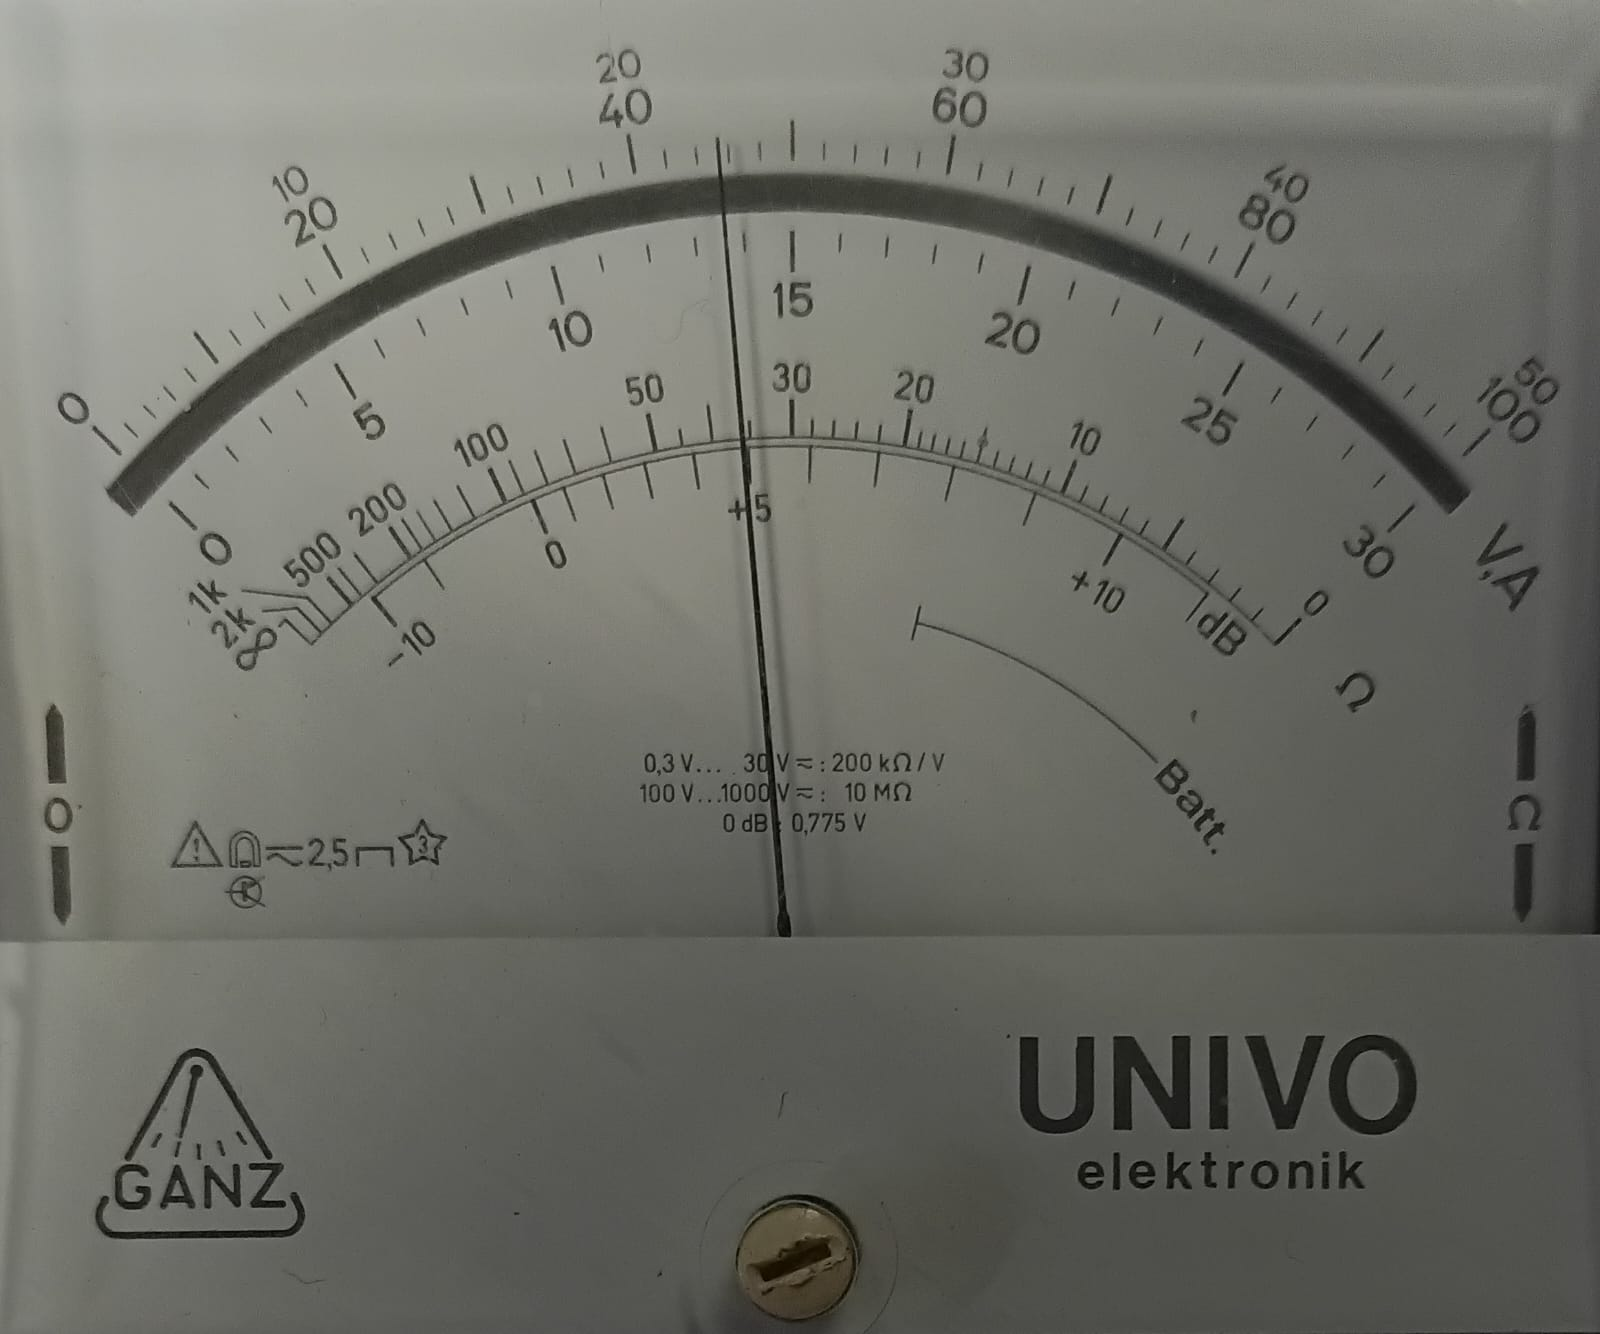
\includegraphics[width=0.5\linewidth]{Imagenes/dBuEnt.jpeg}
    \caption{Voltaje de Entrada en dBu}
    \label{fig:dBuIn}
\end{figure}

    Se midió con el multímetro un valor de salida de $GS_{dBu} = 8.2 \mathrm{dBu}$ y de entrada se midieron unos $GE_{dBu} = 5 \mathrm{dBu}$, por lo tanto la ganancia en tensión del amplificador es de unos $GV = 3.2 \mathrm{dB}$.
Para entender este valor, podríamos expresarlo como un valor de proporcionalidad de la siguiente manera:
\begin{equation*}
\begin{aligned}
     3.2_{dB}=&20\log{\frac{V_s}{V_e}}\\
     \frac{V_s}{V_e}=&10^{3.2/20} = 1.44
\end{aligned}
\end{equation*}

Lo que nos daría por resultado que la señal de salida es aproximadamente $1.44$ veces mas grande que la señal de entrada.

De manera similar al procedimiento anterior, se puede comprobar la ganancia en potencia, tomando y restando los valores de \textbf{dBm} a la entrada y a la salida obtendremos el valor de ganancia de potencia. Como se explico en la sección \ref{sec:Gan} \textbf{dBm} es un valor que expresa que tan grandes es un valor de potencia respecto a $1mW$, los multímetros utilizados no miden esta magnitud, por lo tanto se optó por utilizar la ecuación \ref{eq::PotConVolReferidoa775mV} (derivada a partir de la ecuación principal de \textbf{dBm}), tomando en cuenta la impedancia de entrada, la carga colocada y los valores de \textbf{dBu} ya medidos obtendremos el valor de la ganancia. Recordando la ecuación \ref{eq:Exp4RefGv}
\begin{equation*}
    \begin{aligned}
        GS_{dBm}-Ge_{dBm}=&20\cdot\log{\frac{V_s}{0.775V}} + 10\cdot\log{\frac{600\Omega}{Z_L}}-20\cdot\log{\frac{V_e}{0.775V}} - 10\cdot\log{\frac{600\Omega}{Z_e}}\\
        \\
        =&10\cdot(\log{\frac{V_s^2}{V_e^2}}+\log{\frac{Z_e}{Z_L}})\\
        \\
        =&10\cdot\log{\frac{V_s^2\cdot Z_e}{V_e^2\cdot Z_L}}\\
        \\
        GP_{dB}=&10\cdot\log{\frac{P_s}{P_e}}\\
    \end{aligned}
\end{equation*}

También podemos llegar a la conclusión de que:
\begin{equation}\label{eq:Exp4PotZ}
    GP_{dB}=GV_{dB}-10\log{\frac{Z_L}{Z_e}}
\end{equation}

Nuestro valor de carga sera igual al del experimento 3, ($46.1\Omega$) y el valor medido de la impedancia de entrada en el experimento 2 fue de $1102\Omega$. Tomando estos datos y la ganancia de tensión obtenemos que la ganancia de potencia es de $16.985 \mathrm{dB}$, los valores de potencia de en la salida y entrada fueron de $19.34 \mathrm{dBm}$ y $2.36 \mathrm{dBm}$ respectivamente. Expresando esto como una relación:
\begin{equation}
\begin{aligned}
    16.985_{dB}=&10\log{\frac{P_s}{P_e}}\\
     10^{16.985/10}=&\frac{P_s}{P_e}
\end{aligned}
\end{equation}

Dando como resultado que la potencia de salida es $49.95$ veces más grande que la de entrada.

A continuación se incluye una tabla con todos los datos medidos y calculados en este experimento (tabla \ref{tab:exp4}).

\begin{table}[H]
    \centering
    \scalebox{1}{
    \begin{tabular} {|c|c|c|c|c|c|}
    %{|m{1.5cm}|m{2.7cm}|m{1cm}|p{1.5cm}|m{2.7cm}|}
   
    \hline
          &  &  & \textbf{Incertidumbre} & \textbf{Ganancia} & \textbf{Ganancia} \\
         $f$ & Salida & Entrada & medición de & en \textbf{dB} & en \textbf{veces} \\
          &  &  & en dBu & Salida-Entrada & Salida/Entrada \\
         
         %Frec. Gen. & de $Z_{ent}=R_i$ & en vacío & Para $V_s'=\frac{V_s}{2}$ & medición $R_{e_1}$\\
    \hline
        \multirow{2}{*}{1 kHz} & 8.2 $\mathrm{dBu}$ & 5 $\mathrm{dBu}$ & $\pm0.5 ~dBu$ & 3.2 $\mathrm{dB}$  & 1.44\\
    \cline{2-6}
         & 19.34 $\mathrm{dBm}$ & 2.36 $\mathrm{dBm}$ & $\pm 0.5 ~dBu$ &  16.98 $\mathrm{dB}$ & 49.95 \\
    \hline
        \end{tabular}}
        \def\tablename{Tabla} 
        \caption{Valores obtenidos por mediciones y cálculos}
        \label{tab:exp4}
\end{table}


\subsubsection{Comprobación}

Igual que en el experimento anterior, se realizará una comprobación rápida de los resultados obtenidos. Los datos aquí utilizados fueron tomados de los experimentos 1 y 2, y se respetarán sus nomenclaturas.

Se comenzará con la ganancia en tensión, que en veces, se calcularía así:

\begin{equation*}
    G_V = \cfrac{v_{sal}}{v_{ent}} = \cfrac{v_s'}{v_i} = \cfrac{5.08 [V_{pp}]}{3.08 [V_{pp}]} = 1.649 
\end{equation*}

Esta ganancia de tensión en decibeles sería:

\begin{equation*}
    G_{V_{dB}} = 20 \log (G_V) = 20 \log (1.649) = 4.344 ~dB 
\end{equation*}

Vemos que en ambas hay una diferencia significativa con las calculadas a partir de las mediciones, sin embargo, estas podrían deberse a la incertidumbre en ambas mediciones, ya que esta es bastante alta en el instrumento utilizado.

En el caso de las potencias, realizando un procedimiento similar al realizado en el experimento 3, obtenemos una potencia de entrada de $P_{in}=1.076~mW$. A partir de esta, se calcula la ganancia de potencia en veces y luego en decibeles.

\begin{equation*}
    G_P = \cfrac{P_{sal}}{P_{ent}} = \cfrac{70.25 [mW]}{1.076 [mW]} = 65.288
\end{equation*}

\begin{equation*}
    G_{P_{dB}} = 10 \log (G_P) = 10 \log (65.288) = 18.148 ~dB
\end{equation*}

Nuevamente, los valores medidos no son valores muy exactos en comparación con la medición, pero esto puede ser debido a la suma de errores parciales que como se vió en el experimento 3, viene desde la medición de dBu.


